\documentclass[a4paper, 12pt]{article}

\usepackage[portuges]{babel}
\usepackage[utf8]{inputenc}
\usepackage{amsmath}
\usepackage{indentfirst}
\usepackage{blindtext}
\usepackage{graphicx}
\usepackage[hidelinks]{hyperref}

\author{Igor Abreu da Silva}

\title{Trabalho Final de Sistemas Lineares I}

\begin{document}
	
	\begin{titlepage}
		\begin{center}
			\huge{Universidade Federal do Rio de Janeiro}
			\vspace{95pt}

			\large{Trabalho Final de Sistemas Lineares I}
			\vspace{160pt}
		\end{center}
		
		\begin{flushleft}
			\begin{tabbing}
				Alunos\qquad\qquad\= Igor Abreu da Silva\\
				DRE\> 112053874 \\
				Curso\> Engenharia Eletrônica \\
				Turma\> 2016/1 \\
				Professor\> Natanael Nunes de Moura Junior \\
			
			\end{tabbing}
			
		\end{flushleft}
		
		\begin{center}
			\vspace{\fill}
			Rio de Janeiro, 15 de Julho de 2016
		\end{center}
	\end{titlepage}


	\newpage
	\tableofcontents
	\listoffigures
	\thispagestyle{empty}
	
	\newpage
	\pagenumbering{arabic}
	
	\section{Quest\~{a}o 1}
		\subsection{Determinar a função dos circuito}
			Nesta sessão será resolvida toda a parte necessária para encontra a função/utilidade de cada um dos circuitos. Analisaremos todos os pontos correspondentes aos itens \textbf{(a)}, \textbf{(b)}, \textbf{(c)}, \textbf{(d)}, \textbf{(e)} e \textbf{(f)} do trabalho final. 
			
			
			Serão assumidos aqui que os sistemas encontram-se o zerados no instante $t = 0^{-}$.
			\subsubsection{Circuito 1}
			\begin{figure}[!ht]
				\centering
				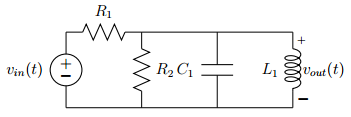
\includegraphics{img/circuito1.png}
				\caption{Circuito 1}	
			\end{figure}			
			Podemos modelar o circuito 1 em relação ao nó após R1. Teríamos a seguinte equação: \\
			\[
				\frac{V_{in} - V_{out}}{R1} - \frac{V_{out}}{R2} - \frac{C\partial V_{out}}{\partial t} - \frac{1}{L} \int V_{out}{\partial t} = 0
			\] 	\\
			Para encontrarmos a E.D.O do circuito, vamos derivar toda esta expressão e separar $V_{out}$ e $V_{in}$, encontrando a seguinte relação:
			\[
				\frac{\partial V_{in}}{\partial t} \left(\frac{1}{R_{1}}\right) = \frac{C \partial^{2} V_{out}}{\partial t^{2}} + \frac{\partial V_{out}}{\partial t} \left(\frac{1}{R_{1}} + \frac{1}{R_{2}} \right) + \frac{V_{out}}{L}
			\] 	\\			
			Em posse da E.D.O, utilizaremos Laplace para encontrar a função de Transferência do Circuito.
			\[
				X(S) \left(\frac{1}{R_{1}}\right) = Y(S)\left(S^{2}C + S \left(\frac{1}{R_{1}} + \frac{1}{R_{2}}\right) + \frac{1}{L} \right) \Rightarrow
			\] 	\\	
			\[
				H(S) = \frac{Y(S)}{X(S)} = \frac{SR_{2}L}{S^{2}\left(R_{1}R_{2}LC\right) + S\left(R_{1}L + R_{2}L\right) + R_{1}R_{2}}
			\] 	\\		
			
			Afim de facilitar os cálculos, tomaremos os seguintes valores para cada elemento do circuito:
			 \begin{itemize}
			 	\item $R_{1} = 10\Omega;$
			 	\item $R_{2} = 100\Omega;$
			 	\item $C = 1F;$
			 	\item $L = 1H;$
			 \end{itemize}		
			 
			Apos aplicar os valores comercias em H(S), temos:
			\[
			H(S) = \frac{100S}{1000S^{2} + 110S + 110}
			\] 	\\					
			
			Utilizando essa função no MatLab para encontrar os polos (quando se zera o denominador), zeros (quando se zera o numerador) e o diagrama de Bode, obtemos o seguintes gráficos:
			
			\begin{figure}[!ht]
				\centering
				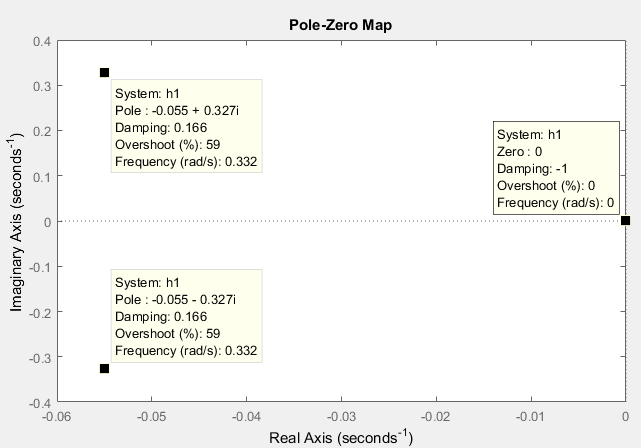
\includegraphics[scale=0.7]{img/1e_circ1.png}
				\caption{Circuito 1 - Polos e Zeros}	
			\end{figure}	
			
			\begin{figure}[!ht]
				\centering
				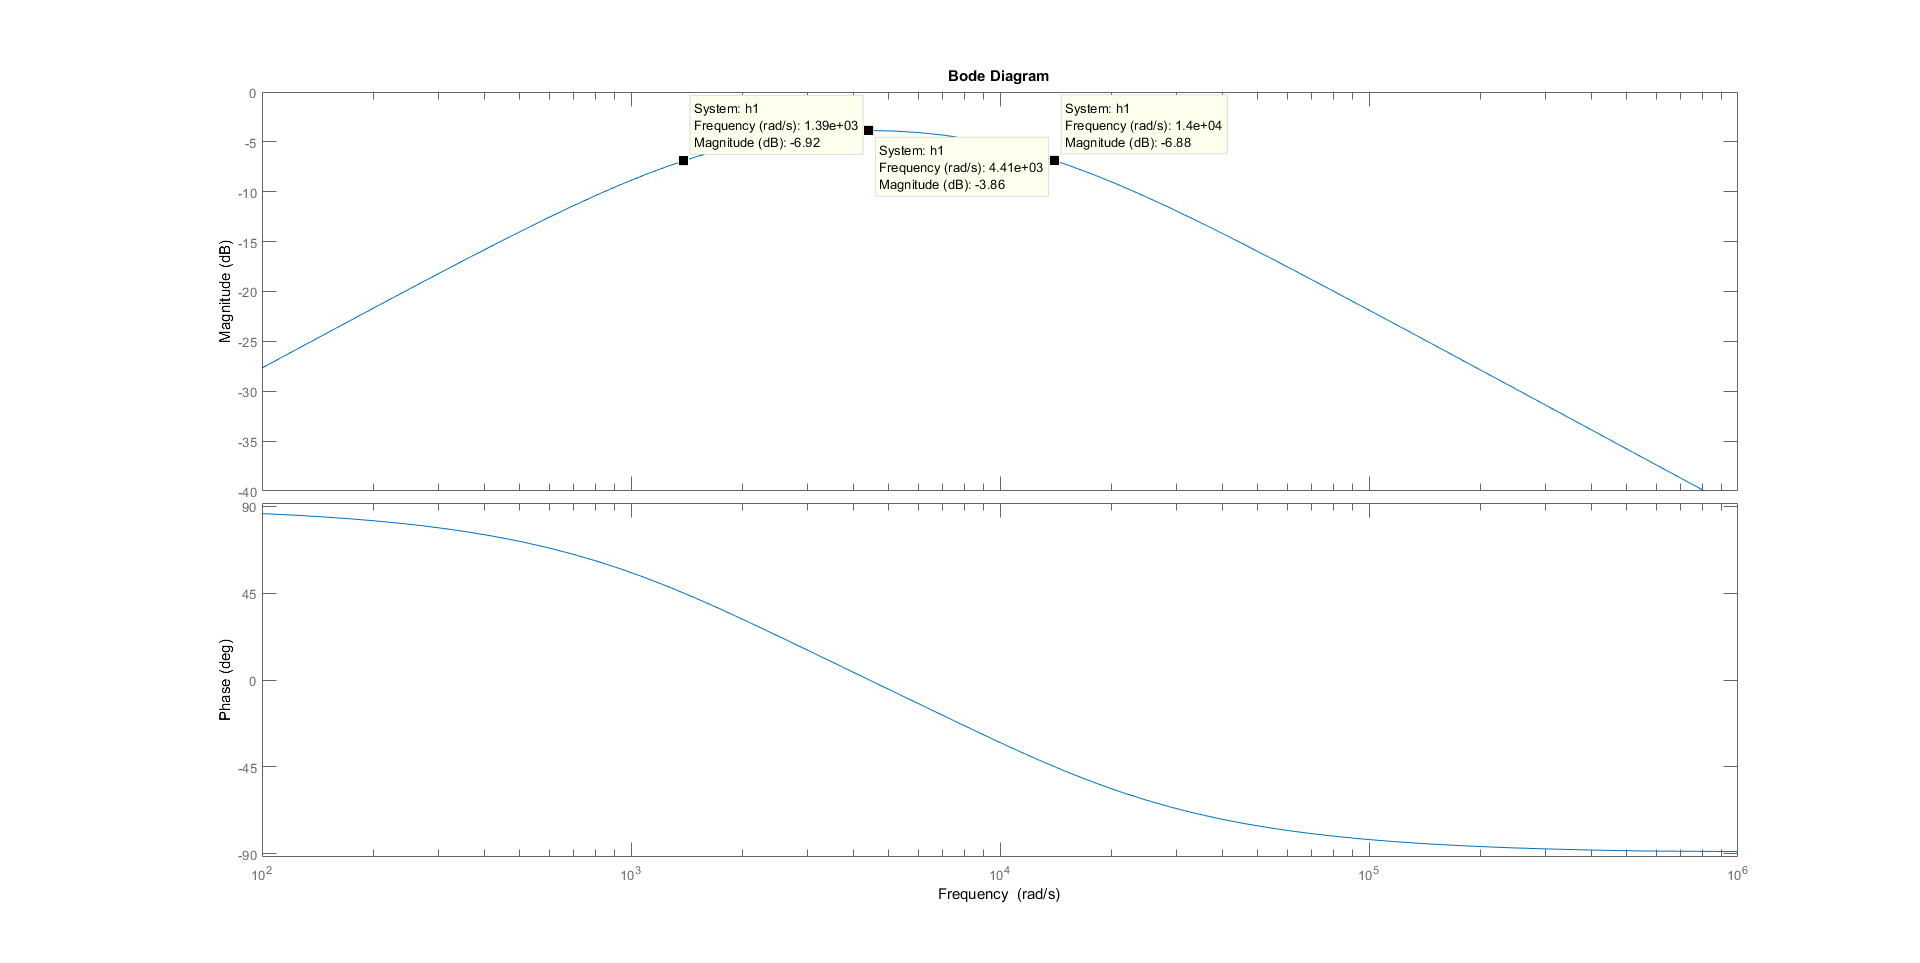
\includegraphics[scale=0.9]{img/1f_circ1.png}
				\caption{Circuito 1 - Diagrama de Bode}	
			\end{figure}						
			\newpage								
			Analisando-se este circuito, pode-se afirmar que o mesmo é um filtro passa faixa operando na largura de banda de aproximadamente 0.11 rad/sec em um intervalo [0.28, 0.39] rad/sec.
			
			
			\subsubsection{Circuito 2}
			\begin{figure}[!ht]
				\centering
				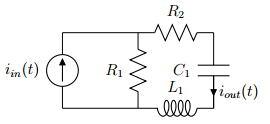
\includegraphics{img/circuito2.png}
				\caption{Circuito 2}	
			\end{figure}			
			
			Para modelarmos utilizaremos as seguintes equações:
			\[				
				 I_{1} = I_{in} - I_{out}
			\] 	\\	
			\[	
				 R_{2}I_{out} + \frac{L \partial I_{out}}{\partial t} - R_{1}I_{1} + \frac{1}{C}\int I_{out}\partial t = 0
			\] 	\\	
			
			Substituindo $I_{1}$ para colocarmos a equação em função de $I_{in}$ e $I_{out}$ e derivando-a para removermos a Integral, temos a E.D.O:
			
			\[	
				\frac{\partial I_{in}}{\partial t}\left(R_{1}\right) = \frac{\partial^{2}I_{out}}{\partial t^{2}}\left(L\right) + \frac{\partial I_{out}}{\partial t}\left(R_{1} + R_{2}\right) + \frac{I_{out}}{C}
			\] 	\\
						
			Transformando essa E.D.O em Laplace, obtemos:
			
			\[	
				X(S)\left(SR_{1}\right) = Y(S)\left(S^{2} + S\left(R_{1} +  R_{2}\right) + \frac{1}{C}\right) \Rightarrow
			\] 	\\			
			\[
			H(S) = \frac{Y(S)}{X(S)} = \frac{S\left(R_{1}C\right)}{S^{2}\left(LC\right) + S\left(R_{1}C + R_{2}C\right) + 1}
			\] 	\\					
			
			Escolhendo os seguintes valores para cada elemento do circuito:
			\begin{itemize}
				\item $R_{1} = 10\Omega;$
				\item $R_{2} = 100\Omega;$
				\item $C = 1F;$
				\item $L = 1H;$
			\end{itemize}	
							
			Encontramos a seguinte função de transferência:
			\[
				H(S) = \frac{10S}{S^{2} + 110S + 1}
			\] 	\\				
			A partir dessa função obtemos os seguintes polos, zeros e diagrama de Bode:
			\begin{figure}[!ht]
				\centering
				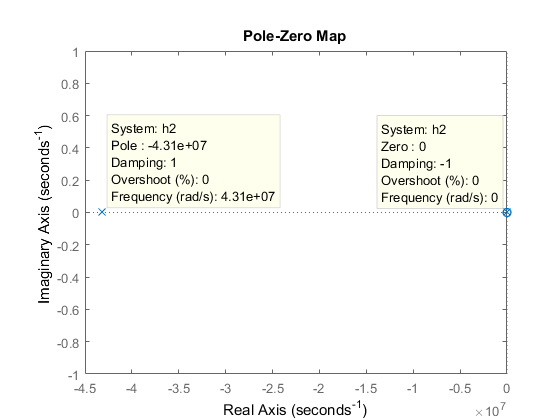
\includegraphics[scale=0.8]{img/1e_circ2.png}
				\caption{Circuito 2 - Polos e Zeros}	
			\end{figure}	

			\begin{figure}[!ht]
				\centering
				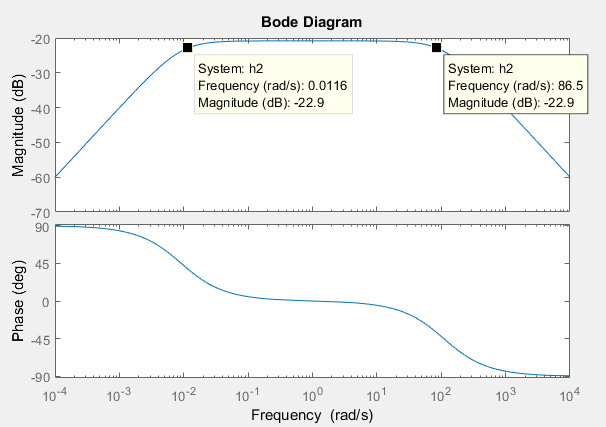
\includegraphics[scale=0.7]{img/1f_circ2.png}
				\caption{Circuito 2 - Diagrama de Bode}	
			\end{figure}			
			\newpage		
			Assim como o circuito da figura 1, temos também um filtro passa faixa que opera nas faixas entre 0.01 rad/seg e 86.5 rad/seg
			\subsubsection{Circuito 3}
			\begin{figure}[!ht]
				\centering
				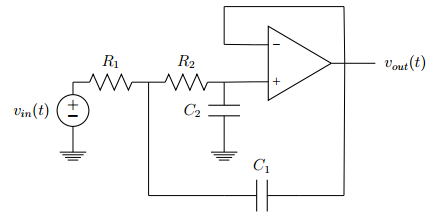
\includegraphics{img/circuito3.png}
				\caption{Circuito 3}	
			\end{figure}			
			
			Este circuito, também conhecido como topologia de Sallen-Key, sabendo que o AmpOp possui impedância infinita em sua entrada, que $V^{-} = V^{+}$, que $V^{-} = V_{out}$ e chamando $V_{a}$ da tensão que passa por $C_{1}$, obtemos:
				
			\[
			V_{a} = V_{out} + R_{2}C_{2}\frac{\partial V_{out}}{\partial t}
			\] 	\\					
			
			Utilizando a lei dos nós entre $R_{1}$ e $R_{2}$ e já substituindo $V_{a}$ por $V_{out}$ temos:
			
			\[
			\frac{V_{in}}{R_{1}} = R_{2}C_{1}C_{2}\frac{\partial^{2} V_{out}}{\partial t^{2}} + \left(C_{2} + \frac{R_{2}C_{2}}{R_{1}}\right)\frac{\partial V_{out}}{\partial t} +  \frac{V_{out}}{R_{1}}
			\] 	\\			
			
			Com esta E.D.O, podemos encontrar a seguinte função de transferência utilizando o mesmo método empregado nos circuitos anteriores, com isso temos:
			
			\[
			H(S) = \frac{1}{S^{2}\left(R_{1}R_{2}C_{1}C_{2}\right) + S\left(R_{1}C_{2} + R_{2}C_{2}\right) + 1}
			\] 	\\					
			
			Utilizando os valores para cada elemento do circuito:
			\begin{itemize}
				\item $R_{1} = 10\Omega;$
				\item $R_{2} = 100\Omega;$
				\item $C_{1} = 2F;$
				\item $C_{2} = 1F;$
			\end{itemize}				

			Encontramos a seguinte função de transferência:
			\[
			H(S) = \frac{1}{2000S^{2} + 110S + 1}
			\] 	\\				
			
			Que nos gera os seguintes polos, zeros e diagrama de Bode:	
			\begin{figure}[!ht]
				\centering
				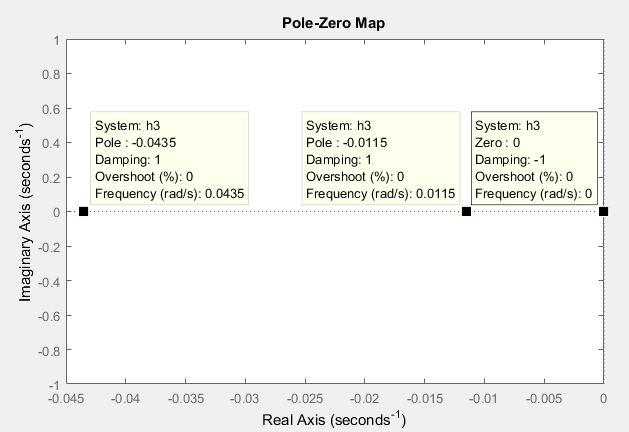
\includegraphics[scale=0.7]{img/1e_circ3.png}
				\caption{Circuito 3 - Polos e Zeros}	
			\end{figure}	
			\newpage
			\begin{figure}[!ht]
				\centering
				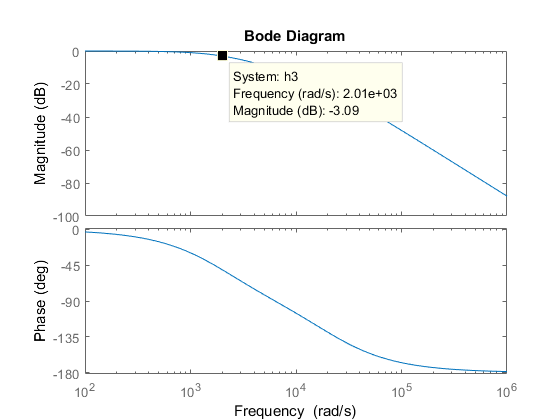
\includegraphics[scale=0.7]{img/1f_circ3.png}
				\caption{Circuito 3 - Diagrama de Bode}	
			\end{figure}			
			Pela a analise do diagrama de Bode, pode-se afirmar que esse circuito é um filtro passa alta com frequência no seu menor polo de 0.01 rad/sec.
			\subsubsection{Circuito 4}
			\begin{figure}[!ht]
				\centering
				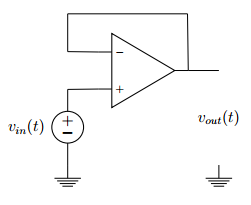
\includegraphics{img/circuito4.png}
				\caption{Circuito 4}	
			\end{figure}		
			
			Esse circuito, conhecido como buffer, é utilizado como um isolador. Como $V_{in}$ é igual a $V_{out}$, sua função de transferência  H(S) = 1. Não existem polos nem zeros para esse circuito e seu diagrama de Bode permanece em 0.
			\begin{figure}[!ht]
				\centering
				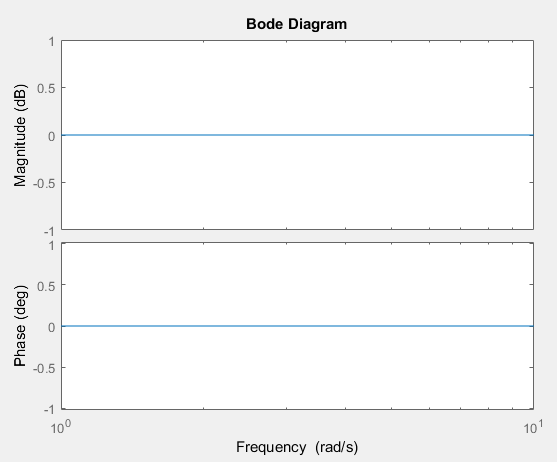
\includegraphics[scale=0.7]{img/1f_circ4.png}
				\caption{Circuito 4 - Diagrama de Bode}	
			\end{figure}				
			\subsubsection{Circuito 5}
			\begin{figure}[!ht]
				\centering
				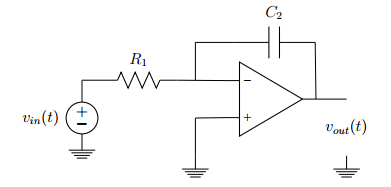
\includegraphics{img/circuito5.png}
				\caption{Circuito 5}	
			\end{figure}							
		\subsection{Item g}		
			\subsubsection{Circuito 1}
			\subsubsection{Circuito 2}
			\subsubsection{Circuito 3}
			\subsubsection{Circuito 4}
			\subsubsection{Circuito 5}		
		\subsection{Item h}		
			\subsubsection{Circuito 1}
			\subsubsection{Circuito 2}
			\subsubsection{Circuito 3}
			\subsubsection{Circuito 4}
			\subsubsection{Circuito 5}		
		\subsection{Item i}			
			\subsubsection{Circuito 1}
			\subsubsection{Circuito 2}
			\subsubsection{Circuito 3}
			\subsubsection{Circuito 4}
			\subsubsection{Circuito 5}		
		\subsection{Item j}		
			\subsubsection{Circuito 1}
			\subsubsection{Circuito 2}
			\subsubsection{Circuito 3}
			\subsubsection{Circuito 4}
			\subsubsection{Circuito 5}		
		\subsection{Item k}		
			\subsubsection{Circuito 1}
			\subsubsection{Circuito 2}
			\subsubsection{Circuito 3}
			\subsubsection{Circuito 4}
			\subsubsection{Circuito 5}		
		\subsection{Item l}			
			\subsubsection{Circuito 1}
			\subsubsection{Circuito 2}
			\subsubsection{Circuito 3}
			\subsubsection{Circuito 4}
			\subsubsection{Circuito 5}								
		\subsection{Item m}			
			\subsubsection{Circuito 1}
			\subsubsection{Circuito 2}
			\subsubsection{Circuito 3}
			\subsubsection{Circuito 4}
			\subsubsection{Circuito 5}										

	\section{Quest\~{a}o 2}
		\subsection{Item a}
		\subsection{Item b}		
		\subsection{Item c}		
		\subsection{Item d}		
		\subsection{Item e}		
		\subsection{Item f}					
		\subsection{Item g}		
		\subsection{Item h}		
		\subsection{Item i}			
		\subsection{Item j}		
		\subsection{Item k}		
		\subsection{Item l}
	
	\section{Quest\~{a}o 3}
		\subsection{Item a}
			\subsubsection{Variando em $\alpha$}
			\subsubsection{Variando em $\beta$}
		\subsection{Item b}	
			\subsubsection{Variando em $\alpha$}
			\subsubsection{Variando em $\beta$}			
		\subsection{Item c}		
			\subsubsection{Variando em $\alpha$}
			\subsubsection{Variando em $\beta$}	
		\subsection{Item d}		
			\subsubsection{Variando em $\alpha$}
			\subsubsection{Variando em $\beta$}	
		\subsection{Item e}		
			\subsubsection{Variando em $\alpha$}
			\subsubsection{Variando em $\beta$}	
		\subsection{Item f}					
			\subsubsection{Variando em $\alpha$}
			\subsubsection{Variando em $\beta$}
		\subsection{Item g}		
			\subsubsection{Variando em $\alpha$}
			\subsubsection{Variando em $\beta$}
		\subsection{Item h}		
			\subsubsection{Variando em $\alpha$}
			\subsubsection{Variando em $\beta$}	
		\subsection{Item i}			
			\subsubsection{Variando em $\alpha$}
			\subsubsection{Variando em $\beta$}
		\subsection{Item j}		
			\subsubsection{Variando em $\alpha$}
			\subsubsection{Variando em $\beta$}	
		\subsection{Item k}	
			\subsubsection{Variando em $\alpha$}
			\subsubsection{Variando em $\beta$}	
	\section{Conclusão}
		
	\newpage
	\section{Referências}
	
	[1] Chapman, S.J. -- Electric Machinery Fundamentals, 4th Edition;
	
	[2] Fitzgerald, A. E. -- Máquinas Elétricas, 2da Edição;
	
\end{document}